\chapter{Revisão Bibliográfica}
\label{stateofart}

  \section{Mercado de Veículos Elétricos}
  \label{stateofart:market}

    O mercado de veículos elétricos, desde o início da década, está aquecido. Nos Estados Unidos, de 2010 à 2014 ouve um aumento de 71\% no volume de vendas (286.390 mil veículos em números absolutos) \cite{fsec-report-ev}. Na China, em 2015, houve um aumento de 4.2 vezes na produção de carros movidos a bateria, e 3.3 vezes quando incluir outras categorias de \ac{EV} \cite{caam-report-ev}.

    Já na União Europeia, de 2013 para 2014 houve um crescimento de 31.5\%, com a venda de 22.6 mil veículos. Embora o crescimento aparente ser grande, está longe de ser maioria no mercado: menos de 1\% da atual frota é constituída de veículos elétricos e a adoção destes depende muito dos incentivos dados em cada país. No contexto Europeu, porém fora da União Europeia, a Noruega se destaca, com uma fatia de 22.5 \% de veículos elétricos nas vendas de 2015. \cite{eaa-report-ev}

    Embora esse mercado apresente potencial, ele ainda depende muito de fatores externos. Isso pode ser visto quando analisamos que as atuais fabricantes possuem poucos modelos, sendo em alguns casos somente uma adaptação de um modelo movido a combustão, pois elas ainda estão testando o mercado e avaliando seus investimentos.

    Alguns fatores influenciam a adoção de veículos elétricos, como:

    \begin{itemize}
      \item Regulamentações exigindo os fabricantes automotores a reduzir emissões de CO2
      \item Incentivos fiscais e financeiros para a aquisição de veículos e operações relacionadas
      \item Preços de combustíveis
      \item Custos de baterias e evolução da tecnologia
      \item Infraestrutura do ecossistema de veículos elétricos (pontos de carregamento e manutenção)
    \end{itemize}

    Alguns países Europeus, como a Alemanha, já afirmaram que desejam abolir vendas de veículos a combustão \cite{forbes-news-germany}. Outros países planejam seguir a mesma linha, o que força as fabricantes a iniciarem pesquisas na área e desenvolver as tecnologias relacionadas a esse mercado.

  \section{Modos de Operação de \ac{EVSE}}
  \label{stateofart:modes}

    \subsection{Modos Europeus}
    \label{stateofart:modes:europe}

      Os modos de carregamento europeus seguem o padrão IEC 62196 \cite{iec-62196}, que apresenta quatro modos de operação.

        \subsubsection{Modo 1 - Carregamento Lento}
        \label{stateofart:modes:europe:mode1}

        Utiliza plug de tomada residenciais, o qual não pode exceder 16 A de corrente e 250 V \ac{CA} monofásica ou 480 V AC de tensão trifásica. Normalmente ele toma de 6 à 8 horas para carregar completamente o veículo, o que é considerado um carregamento lento. Como é utilizada uma tomada comum, não é necessária uma \ac{EVSE} para fazer o controle desse carregamento. Porém, como esse padrão utiliza uma proteção diferencial e requer uma proteção aterrada na residência, muitos países não o adotam, visto que há boa parte das residências não possuem aterramento.

        \subsubsection{Modo 2 - Carregamento Lento}
        \label{stateofart:modes:europe:mode2}

        É necessária uma caixa de controle no plug ou no cabo, sendo que esta faz a comunicação com o veículo por meio de \ac{PWM}. Graças a essa comunicação, o carro pode informar o status de sua bateria e assim o carregamento pode ser adaptado de acordo com esse dado. Ele utiliza o mesmo plug do Modo 1 e possui as mesmas limitações elétricas de tensão, porém permite um máximo de até 32 A de corrente. Dentro dessa caixa de controle há também um circuito de proteção, o que permite o uso desse modo em locais não aterrados. Ele é utilizado em alguns locais públicos da Europa e é considerado uma solução de transição nos EUA.

        \subsubsection{Modo 3 - Carregamento Rápido CA}
        \label{stateofart:modes:europe:mode3}

        O cabo é conectado à uma \ac{EVSE}, sendo que ela precisa estar habilitada à comunicação PWM e possuir uma proteção elétrica. O carregamento pode ser ajustado de acordo com os dados recebidos pelo pino de controle da estação, o que possibilita o ajuste do carregamento (lento ou rápido). Com o uso de 400 V trifásico com 63 A de corrente, é possível carregar certos carros em menos de uma hora. Esse modo está se tornando cada vez mais comum, porém requer um equipamento de eletrônica de potência adequado à tensão e corrente máxima desejadas. O desenvolvimento desse modo possui um grande investimento da empresa japonesa \textit{CHAdeMO}, sendo as vezes referido como padrão \textit{CHAdeMO} \cite{ieee-review-evse}.

        \subsubsection{Modo 4 - Carregamento Rápido CC}
        \label{stateofart:modes:europe:mode4}

        Este modo ultra-rápido permite tensões de 400 V e corrente de 200 A, utilizando \ac{CC} para tal. Esse modo requer um inversor para converter a entrada da rede de \ac{CA} para \ac{CC}. Estações que permitem carregamento no modo 4 custam muito mais caro que estações modo 3, sem contar que o projeto precisa de uma atenção especial no quesito segurança, porém ela está se tornando cada vez mais atrativa devido a velocidade de seus carregamentos.

    \subsection{Modos Americanos}
    \label{stateofart:modes:us}

      \begin{itemize}
        \item Nível 1: assim como o modo 1 europeu, utiliza um plug residencial (americano) para o carregamento, fornecendo até 120 V AC ao veículo.
        \item Nível 2: pode fornecer 240 ou 208 V AC e de 20 à 100 A. Em instalações residenciais, normalmente acaba limitado à 30 A, podendo oferecer até 7.2 kW de potência. Este é o modo mais comum de instalação em residências americanas.
      \end{itemize}

      Há ainda modos de corrente contínua, sendo que esses são idênticos ao Modo 4 Europeu.

    \subsection{Outros modos}
    \label{stateofart:modes:other}

      \subsubsection{Indução}
      \label{stateofart:modes:other:induction}

        O veículo pode ser carregado sem precisar estar conectado à uma estação, o que oferece maior segurança e comodidade para o motorista. Ele pode ser carregado de três maneiras

        \begin{itemize}
          \item Estática: veículo é carregado enquanto está estacionado
          \item Quasi-estática: o veículo é carregado enquanto há pessoas dentro, porém em locais específicos (parado no trânsito, por exemplo)
          \item Dinamicamente: enquanto o veículo está em movimento, como em uma rodovia
        \end{itemize}

        Ainda há muita pesquisa nesse modo, principalmente devido a sua baixa eficiência quando comparado aos modos cabeados.

      \subsubsection{Troca de Baterias}
      \label{stateofart:modes:other:swap}

        Há a possibilidade de carregamento por troca de baterias, onde o veículo para em uma estação e um sistema automatizado remove a bateria atual do carro e a substitui por uma carregada. Essa opção oferece segurança para o motorista e não sofre do problema de eficiência do carregamento por indução.

      \subsubsection{Tesla Supercharge}
      \label{stateofart:modes:tesla}

        Nos modos cabeados, ainda há o modo proprietário da fabricante Tesla, o \textit{Tesla Supercharge}, que permite o carregamento de 50\% da bateria do Tesla S (85kWh) em menos de 20 minutos. Para possibilitar tal carregamento, os carregamentos são realizados em corrente contínua, assim como o Modo 4 Europeu.

  \section{Padrões de Conectores}
  \label{stateofart:plugs}

      Diversos tipos de conectores estão disponíveis hoje no mercado. Um dos padrões mais aceitos para o carregamento lento é o Tipo 2 - \textit{Mennekes}. Ele já foi submetido para se tornar padrão oficial desse tipo de carregamento na Europa \cite{mckinsey-report-ev}.

      Para carregamentos rápidos porém, existem três conectores que são bastante usados: o CHAdeMO, o CCS Combo e o Tesla Supercharger. Normalmente, as estações fornecem o conector Mennekes e uma ou duas opções de carregamento rápido, o que é similar ao que ocorre em estações para veículos movidos a combustão (gasolina e álcool no mesmo posto).

      \subsection{Tipo 2 - Mennekes}
      \label{stateofart:plugs:mennekes}

        Proposto pela empresa Mennekes, permite carregamentos \ac{CA} monofásicos/trifásicos e \ac{CC}, além de ser retrocompatível com conectores Tipo 1, mesmo possuindo 7 pinos (contra 5 do tipo 1). Ele permite que a corrente flua de forma bi-direcional, o que permite que os \ac{EV} possam fornecer energia para a estação, previsto no modelo de \textit{Vehicle-to-Grid}. Ele é muito utilizado em carregamentos de modo 1 e modo 2, porém no modo 3 outros conectores são necessários.

        \begin{figure}[H]
          \begin{center}
            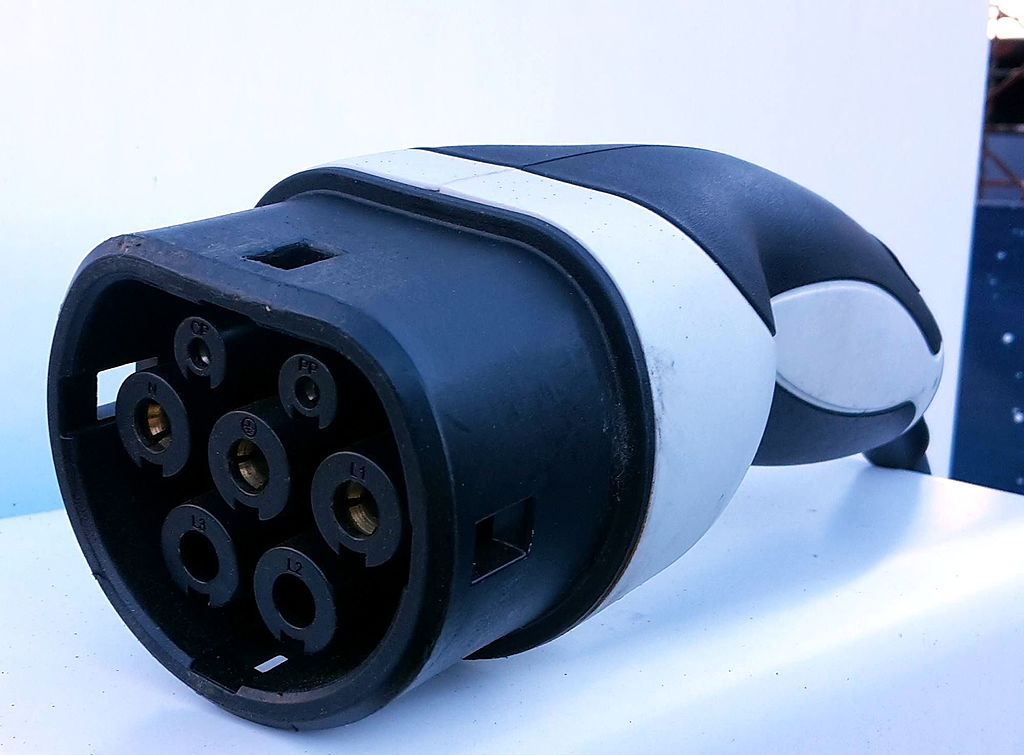
\includegraphics[width=0.50\textwidth,natwidth=1024,natheight=755]{assets/images/connectors-mennekes.jpg}
            \caption{Conector Mennekes}
            \label{fig:mennekes}
          \end{center}
        \end{figure}

      \subsection{CCS Combo}
      \label{stateofart:plugs:combo}

        Permite carregamentos rápidos em \ac{CC} e \ac{CA}. O conector possui uma parte eletrônica para garantir a segurança do usuário, onde o conector checa se foi conectado corretamente antes de a operação, além de previnir a desconecção durante o carregamento ou antes do pagamento ser efetivado.

        \begin{figure}[H]
          \begin{center}
            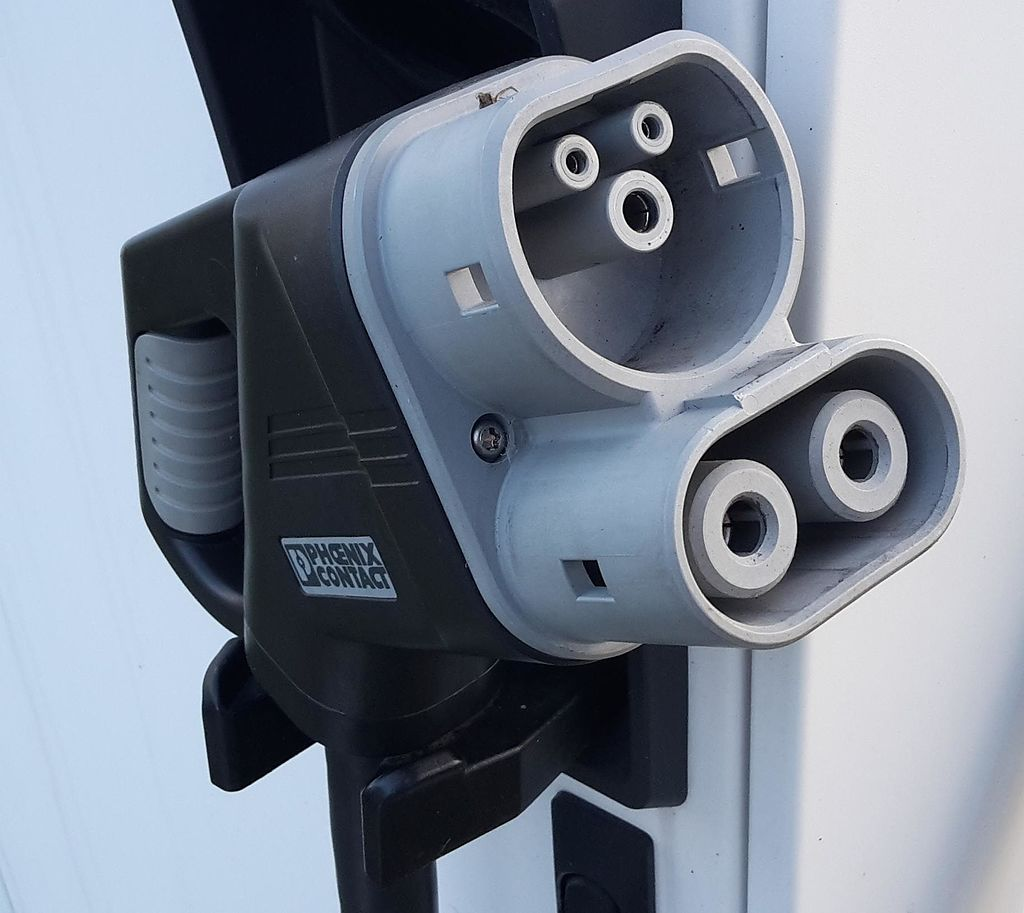
\includegraphics[width=0.40\textwidth,natwidth=1024,natheight=973]{assets/images/connectors-combo.jpg}
            \caption{Conector CCS Combo}
            \label{fig:combo}
          \end{center}
        \end{figure}

      \subsection{CHAdeMO}
      \label{stateofart:plugs:chademo}

        Utilizado junto ao carregamento modo 3 e 4, foi o primeiro conector que possibilitou carregamentos rápidos e \ac{CC}. Hoje, porém, outros padrões como o CCS Combo estão oferecendo um suporte satisfatório para carregamentos rápidos \cite{ieee-review-evse}. Visto a preocupação da CHAdeMO com segurança e o alto nível de tensão, esse conector possui 10 pinos.

        \begin{figure}[H]
          \begin{center}
            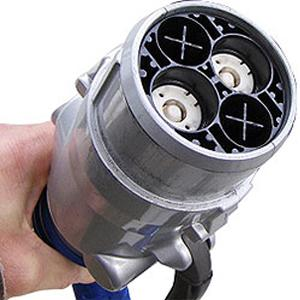
\includegraphics[width=0.35\textwidth,natwidth=300,natheight=300]{assets/images/connectors-chademo.jpg}
            \caption{Conector CHAdeMO}
            \label{fig:chademo}
          \end{center}
        \end{figure}

      \subsection{Tesla Supercharger}
      \label{stateofart:plugs:tesla}

        Fornecido pela Tesla Motors, ele foca em carregamentos rápidos em \ac{CC} - modo 4 - e empresas como Nissan e BMW já negociam um acordo com a Tesla para a utilização do conector em seus veículos, permitindo que sua frota utilize a infra-estrutura de carregamentos Tesla Supercharge.

        \begin{figure}[H]
          \begin{center}
            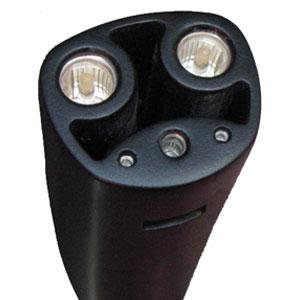
\includegraphics[width=0.35\textwidth,natwidth=300,natheight=300]{assets/images/connectors-tesla.jpg}
            \caption{Conector Tesla Supercharger}
            \label{fig:tesla}
          \end{center}
        \end{figure}

  \section{Protocolo OCPP}
  \label{stateofart:ocpp}

    As estações de carregamento normalmente se comunicam com um servidor central, que pode gerenciar N estações. Para tal tarefa, é necessário um protocolo de comunicação. Embora ainda não exista um padrão oficial, o \ac{OCPP} é um padrão \textit{de facto} e já existem esforços para o tornar um padrão oficial junto a \ac{OASIS} \cite{ocpp-news-standardization}.

    Mantido e criado pela \ac{OCA}, o OCPP está presente em mais de 50 países. Na Europa, todas estações comercializadas precisam ser compatíveis com o OCCP e, na América, o interesse da indústria está aumentado \cite{forbes-news-ocpp}.

    O protocolo prevê um sistema central que recebe dados de N estações. Caso for necessário, o sistema central pode atuar sob \ac{EVSE} específicas com ações como reservar a estação, cancelar algum carregamento ou até desligá-la. Caso a estação perca conectividade, o protocolo prevê que ela deve funcionar de modo autônomo, somente registrando alguns dados para envio posterior (início e finalização de carregamentos) \cite{ocpp-spec-15}.

    As requisições da versão 1.5 podem ser via SOAP ou WebSocket, enquanto a versão 1.6 já adiciona suporte a JSON. A versão 2.0, em desenvolvimento, tem em mente a padronização do protocolo e retrocompatibilidade com versões anteriores.
